%!TEX encoding = UTF-8 Unicode
% TODO: Druckversion: ',openright,twoside'
\documentclass[12pt,a4paper,pointednumbers,abstracton]{scrartcl}
%\usepackage[applemac]{inputenc} % Mac-Umlaute direkt verwenden öäüß
%\usepackage[isolatin]{inputenc} % PC-Umlaute direkt verwenden 
\usepackage[utf8]{inputenc} % Unicode funktioniert unter Windows, Linux und Mac
\usepackage[T1]{fontenc}
\usepackage{ngerman}
\usepackage{graphicx}
\usepackage{hyperref}\urlstyle{rm}
\usepackage{times}
\usepackage{tikz}
\usepackage[scaled]{helvet}
\usepackage{a4wide}
\usepackage{rotating}
\usepackage[T1]{fontenc}
\usepackage{color}
\usepackage{listings}

% Fonts
\newcommand{\changefont}[3]{
\fontfamily{#1} \fontseries{#2} \fontshape{#3} \selectfont}

% Colors
\definecolor{DarkPurple}{rgb}{0.4,0.1,0.4}
\definecolor{DarkCyan}{rgb}{0.0,0.5,0.4}
\definecolor{LightLime}{rgb}{0.4,0.6,0.5}
\definecolor{Blue}{rgb}{0.0,0.0,1.0}

% Listings
\lstdefinestyle{PHP}
{
language=PHP,
numbers=left,
firstnumber=1,
stepnumber=1,
numberfirstline,
numberstyle=\tiny\sffamily,
tabsize=5,
captionpos=b,
aboveskip=1em,
belowskip=1em,
columns=flexible,
xleftmargin=2em,
xrightmargin=1em,
frame=single,
frameround=ftft,
commentstyle=\bfseries\itshape\color{LightLime},
keywordstyle=\bfseries\color{DarkPurple},
basicstyle=\footnotesize\ttfamily,
stringstyle=\color{Blue},
showstringspaces=false,
}

\lstdefinestyle{InlinePHP}
{
language=PHP,
columns=flexible,
basicstyle=\bfseries\footnotesize\ttfamily\color{DarkCyan},
showstringspaces=false,
}

% Blank Pages
\newcommand{\blankpage}{
\newpage
\thispagestyle{empty}
\null
\vfill
\begin{center}
	This page is intentionally left blank.
\end{center}
\newpage
}

% inline circled numbers
\newcommand*\circled[1]{\tikz[baseline=(char.base)]{
\node[shape=circle,draw,inner sep=2pt] (char) {#1};}}
            

% inline code
\newcommand{\code}[1]{\small\lstinline[style=InlinePHP]!#1!\normalsize}
%\newcommand{\code}[1]{\scriptsize\texttt{#1}\normalsize}

% deactivate block
\newcommand{\deactivate}[1]{}

\hyphenation{InfRZ OAuth Web-anwendung Web-anwendungen}

\sloppy
\setlength{\parindent}{0em}
\setlength{\parskip}{1.2ex plus 0.5ex minus 0.5ex}
\pagestyle{plain}

\title{Realisierung eines Single-Sign-On-Dienstes für das Informatik-Netz}
\author{Senad Ličina}
\date{\today}

\begin{document}
\pagenumbering{Roman}

%%%%%%%%%% Deckblatt
\thispagestyle{empty}
\addcontentsline{toc}{subsection}{Muster des Deckblatts}
\begin{center}\Large
Universität Hamburg \par
Fachbereich Informatik
\vfill
Bachelorarbeit
\vfill
{\Large\textsf{\textbf{Realisierung eines Single-Sign-On-Dienstes\\ für das Informatik-Netz}}\par}
\vfill
vorgelegt von 
\par\bigskip
Senad Ličina \par
geb. am 23.03.1988 in Berane (MNE) \par
Matrikelnummer 5945457 \par
Studiengang Informatik \par
\vfill
eingereicht am \today
\vfill 
Betreuer: Dipl.-Wirtsch.-Inf. Dominik Herrmann \par
Erstgutachter: Prof. Dr.-Ing. Hannes Federrath \par
Zweitgutachter: Dr. Andreas Günter
\end{center}
%%%%%%%%%% Ende Deckblatt

\deactivate{
%%%%%%%%%% Deckblatt Hübsch
\changefont{cmss}{m}{n}
\thispagestyle{empty}

\begin{center}
    \Large{Bachelorarbeit}\\
    \vspace{1em}
    \Huge{\textbf{
        OAuth InfRZ\\
        \vspace{0.2em}
    }}
    \Large{
        Realisierung eines Single-Sign-On-Dienstes\\ für das Informatik-Netz
    }

    \vspace{4cm}
    \normalsize
    vorgelegt von\\
    \Large
    Senad Ličina\\
    \vspace{0.2em}
    \normalsize
    geb. am 23.03.1988 in Berane (MNE)\\
    Matrikelnummer 5945457\\
    Studiengang Informatik\\
    \vspace{1em}
    eingereicht am \today\\
    \vspace{6em}
    
    Betreuer: Dipl.-Wirtsch.-Inf. Dominik Herrmann \\
    Erstgutachter: Prof. Dr.-Ing. Hannes Federrath \\
    Zweitgutachter: Dr. Andreas Günter
\end{center}

\vfill

\footnotesize
\parbox{0.5\linewidth}{
  \parskip 0.4em

  Arbeitsbereich Sicherheit in Verteilten Systemen (SVS)

  Fachbereich Informatik

  Universität Hamburg
}
\hfill
\parbox{4.2cm}{
  \includegraphics[height=2.0cm]{img/logo_fbi}
  \hfill
  \includegraphics[height=2.0cm]{img/logo_uhh}
}

\addtolength{\voffset}{2cm}

%%%%%%%%%% Ende Deckblatt hübsch
}

\normalsize
\changefont{ppl}{m}{n}
%\rmfamily
\newpage
%\blankpage
\setcounter{page}{1}
%\addtolength{\voffset}{-2cm} % Deckblatt Hübsch
\section*{Aufgabenstellung}

Im Informatik-Rechenzentrum der Universität Hamburg werden die Benutzerdaten aller Mitarbeiter und Studenten in einem LDAP-Verzeichnis (MS ActiveDirectory) vorgehalten.

Im Rahmen einer Bachelorarbeit ist auf Basis dieser Infrastruktur ein webbasierter Single-Sign-On-Dienst (SSO-Dienst) zu implementieren, der von verschiedenen \mbox{(Web-)Anwendungen} genutzt werden kann. Dies erlaubt es den Entwicklern von Web-Anwendungen, den sensiblen Prozess der Benutzerauthentifizierung, bei der das vom Benutzer eingegebene Passwort übermittelt und geprüft werden muss, an den SSO-Dienst auszulagern.

Die Nutzung des SSO-Dienstes soll möglichst über (Standard-)Schnittstellen, etwa OAuth 2.0, möglich sein. Im Rahmen der Bachelorarbeit ist ein Entwurf für den Dienst anzufertigen und ein Prototyp zu implementieren. Weiterhin sind Beispiel-Implementierungen sowie eine leicht verständliche Dokumentation mit Tutorial-Charakter für die wesentlichen Entwicklungsumgebungen (z.B. PHP, Java, Ruby on Rails) anzufertigen. Die Umsetzung muss hohen Sicherheitsanforderungen genügen.

\newpage
%\blankpage
\section*{Zusammenfassung}



Für den eiligen Leser sollen auf etwa einer halben, maximal einer Seite die wichtigsten Inhalte, Erkenntnisse, Neuerungen bzw. Ergebnisse der Arbeit beschrieben werden. 

Durch eine solche Zusammenfassung (im engl. auch Abstract genannt) am Anfang der Arbeit wird die Arbeit deutlich aufgewertet. Hier sollte vermittelt werden, warum der Leser die Arbeit lesen sollte.

\newpage
\tableofcontents

\newpage
\pagenumbering{arabic}
\setcounter{page}{1}
\section{Einleitung}
\label{sec:einleitung}

Ein \textbf{Single-Sign-On-Dienst (SSO-Dienst)} bietet dem Benutzer die Möglichkeit nach einer einmaligen Authentifizierung auf mehrere Ressourcen und Dienste zuzugreifen.
Der Einsatz eines SSO-Dienstes soll die Benutzung komfortabler und sicherer gestalten.
In \cite{Hur97} wird Single-Sign-On definert, damit verbundene Implementierungsschwierigkeiten erörtert und zwischen unterschiedlichen Modellen unterschieden.

Im Zeitalter des Web 2.0\footnote{vgl. Tim O'Reilly: What Is Web 2.0. \url{http://oreilly.com/web2/archive/what-is-web-20.html} (Zugriff am 26.02.2013)} wird ein simpler und einheitlicher Autorisierungsmechanismus immer wichtiger.
Besonders in den letzten Jahren hat sich das offene Protokoll \textbf{OAuth} zu diesem Zweck durchgesetzt.
Obwohl OAuth primär der Autorisierung dient, bieten die meisten großen Web-Portale OAuth zur Authentifizierung der Benutzer und Autorisierung dritter Anwendungen an.
Der Einsatz eines SSO-Dienstes erleichtert die Entwicklung weiterer unabhängiger Dienste und kann deren Sicherheit durch die Übernahme sicherheitsrelevanter Kernfunktionen erhöhen.
Neben hohen Sicherheitanforderungen, denen ein solcher Dienst entsprechen muss, sollte er auch vertrauenswürdig, benutzerfreundlich, selbsterklärend, wart- und erweiterbar sein.

Das Informatik Rechenzentrum der Universität Hamburg benutzt zur Verwaltung und Bereitstellung der Benutzerdaten den Verzeichnisdienst \textbf{Active Directory}.
Durch das Ansprechen des Active Directory wird es Benutzern ermöglicht sich mit ihren Informatik-Rechenzentrum-Anmdeldedaten (Credentials)\footnote{die Benutzerkennung und das dazugehörige Passwort} zu authentifizieren.
Diese Authentifizierung kann gegen alle beim OAuth-Dienst angemeldeten Dienste erfolgen.
Desweiteren können Benutzer angemeldete Dienste für den Zugriff auf ihre Informationen autorisieren.
Der Einsatz eines OAuth-Dienstes entkoppelt die Authentifzierung von der Funktionalität weiterer Dienste und kann so deren Sicherheit erhöhen.
Eine Reduzierung der erforderlichen Authentifizierungen\footnote{und damit die Anzahl der Übertragungen der sensiblen Credentials} wirkt sich ebenfalls positiv auf die Sicherheit aus.
Ein selbsterklärender, transparenter und einheitlicher Authentifizierungs- und Autorisierungsvorgang kann zu mehr Vertrauen bei den Benutzern führen.

Bei diesem Dokument handelt es sich um einen Teil der Dokumentation zu OAuth InfRZ, ein vom Autor im Frühjahr 2013 entwickelter SSO-Dienst für den Fachbereich Informatik der Universität Hamburg.
OAuth InfRZ ist Bestandteil dieser Bachelorarbeit.

Dieses Dokument ist wie folgt aufgebaut:

\deactivate{
Kapitel \ref{sec:einleitung} liefert eine \textbf{Einleitung} in die Materie und soll OAuth InfRZ in einen Kontext bringen.
Es wird die Relevanz eines SSO-Dienstes erörtert, eine Implementierungsmöglichkeit skizziert und eine Zusammenfassung zu jedem Kapitel gegeben.
}

Kapitel \ref{sec:basics} bringt den Leser auf den zum Verständnis der Arbeit erforderlichen Wissensstand, indem es wichtige \textbf{Grundlagen} und die damit verbundenen Fragestellungen klärt.
Es wird auf Authentifizierung, Autorisierung, ein Verschlüsselungsprotokoll für Netzwerkübertragungen und den vom Fachbereich Informatik genutzten Verzeichnisdienst eingegangen.

In Kapitel \ref{sec:oauth} wird \textbf{OAuth} erklärt und seine Funktionsweise beschrieben.
Es werden die Vorteile von OAuth gegenüber herkömlicher Authentifizierung erörtert, die Versionen gegenübergestellt, der OAuth2 Workflow skizziert und die Sicherheit bewertet.

Kapitel \ref{sec:oauth-infrz} enthält eine technische Dokumentation zu \textbf{OAuth InfRZ}.
Zunächst werden die Anforderungen an ein solches System skizziert und die Benutzung von OAuth InfRZ erklärt.
Um die Einarbeitungszeit von weiteren Entwicklern zu reduzieren, werden die eingesetzten Werkzeuge und Konzepte vorgestellt und komplexe Besonderheiten zur technischen Realisierung ausgeführt.
Außerdem wird die Client-Library vorgestellt und ein Ausblick mit Aufwandsbewertung auf die Erweiterbarkeit von OAuth InfRZ geboten.

%\begin{quote}
%\textbf{Untersuchungsverlauf} \emph{(pro Kapitel ein – kurzer – Absatz mit Verweis auf die Kapitelnummer);}\\
%hier wird geklärt, was Inhalt der einzelnen Kapitel ist. Neue inhaltliche oder methodische Aspekte sollten hier nicht mehr vorkommen, hier geht es nur noch um das Wie, nicht mehr um das Was. (\textbf{Kontrollfrage: „Wie wird vorgegangen?“})
%\end{quote}

\newpage
\section{Grundlagen}
\label{sec:basics}

In diesem Kapitel werden für das Verständnis dieses Dokuments notwendige Konzepte und Technologien diskutiert.
Zunächst werden Authentifizierung und Autorisierung unterschieden.
Dann wird das Verschlüsselungsprotokoll Transport Layer Security (TLS) erklärt, seine Funktionsweise skizziert und seine Sicherheit erörtert.
Außerdem werden der Verzeichnisdienst Active Directory (AD) und das Lightweight Directory Access Protocol (LDAP) erklärt und in einen Zusammenhang gebracht.

% Authentication / Authorization
\subsection{Authentifizierung und Autorisierung}

Als \textbf{Authentifizierung} wird die Verifizierung behaupteter Eigenschaften bezeichnet.\footnote{vgl. \cite[Section 8.7]{TW10}}
Im speziellen ist bei einer Authentifizierung im World Wide Web (WWW) meist die Prüfung und Erteilung einer Zugangsberechtigung gemeint.
Dies kann durch den Login eines Benutzers bei einer Webanwendung geschehen.
Der Benutzer authentisiert sich bei der Webanwendung indem er sein Passwort übermittelt.
Im Gegenzug authentifiziert die Webanwendung den Benutzer.

Die \textbf{Autorisierung} ist das Einräumen von Zugriffsrechten für einen Benutzer oder ein Programm.
Eine Autorisierung setzt eine erfolgreichen Authentifizierung vorraus.

\begin{quote}
\emph{,,As an aside, some people confuse authorization with authentication.
Authentication deals with the question of whether you are actually communicating with a specific process.
Authorization is concerned with what that process is permitted to do.''}
\begin{flushright}
\small{-- \cite{TW10} Section 8.7}
\end{flushright}
\end{quote}

% TLS
\subsection{Transport Layer Security}

Bei \textbf{Transport Layer Security (TLS)}\footnote{auch bekannt unter der Vorgängerbezeichnung \emph{Secure Sockets Layer (SSL)}} handelt es sich um ein \emph{hybrides Verschlüsselungsprotokoll}.\footnote{vgl. \cite[Hannes Federrath, Andreas Pfitzmann: ,,IT-Sicherheit''. Kapitel 2.4 (S. 279-281)]{WK06}}
Es wird von der Internet Engineering Task Force (IETF) gepflegt, welche im August 2008 mit \cite{RFC5246} die aktuellste Version \emph{TLS 1.2} vorstellte.

Im Transmission Control Protocol/Internet Protocol Reference Model (TCP/IP-Modell)\footnote{vgl. \cite[Section 1.4.2]{TW10}} wird TLS zwischen der Transport- und Anwendungsschicht angesiedelt.
\cite[Section 8.9.3]{TW10} gliedert es in eine eigene \emph{,,Security''} Schicht.
Im Open Systems Interconnection Reference Model (OSI-Modell)\footnote{vgl. \cite[Section 1.4.1]{TW10}} wird es in die Kommunikationssteuerungsschicht gegliedert.\footnote{vgl. \cite[Section 12.4]{Sin12}}
Es wird hauptsächlich zur Sicherung von HTTP-Verbindungen eingesetzt.

\subsubsection{Funktionsweise \& Verschlüsselung}

Als ein \textbf{hybrides Verschlüsselungsprotokoll} setzt TLS sowohl auf \emph{symmetrische} als auch auf \emph{asymmetrische} Verschlüsselung.
Im ersten Schritt handeln die Kommunikationspartner die Sicherheitsparameter durch asymmetische Verschlüsselungsverfahren aus und haben die möglichkeit sich durch Zertifikate zu authentifizieren.
In der Regel authentifizieren sich nur die Server.
Der Inhalt der Datenübertragung wird dann mit dem ausgehandelten Schlüssel symmetrisch verschlüsselt.
Um eine höhere Sicherheit gewährleisten zu können, werden für jede Übertragung neue Sicherheitsparameter ausgehandelt.
Die Nachrichtenintegrität wird durch Message Authentication Codes (MAC)\footnote{vgl. \cite{TW10} Section 8.6.1} gewährleistet.
Von Zertifizierungsstellen (Certificate Authorities) signierte Zertifikate dienen als Nachweis der Identität.

\subsubsection{Sicherheit}
\label{sec:basics-security}

Obwohl \emph{TLS 1.2} als hinreichend sicher gilt, steht die Sicherheit von TLS unter Kritik.
Die meisten Browser unterstützen bislang nur die unter anderem durch \emph{BEAST attacks}\footnote{vgl. \cite{DR11}} angreifbare Version \emph{TLS 1.0}.
Als Grund für die geringe Verbreitung von \emph{TLS 1.2} nennt \cite{Rit12} den zu großen Implementierungsaufwand für einen zu geringen Mehrwert.
Selbst wenn \emph{TLS 1.2} benutzt werden soll, ist es möglich die Sicherheitslücken von \emph{TLS 1.0} mithilfe einer \emph{downgrade attack} auszunutzen, da bei einem gescheiterten Handshake auf \emph{TLS 1.0} zurückgegriffen wird.

Neben dem Nachteil der geringen Verbreitung von \emph{TLS 1.2} stehen vorwiegend die Zertifizierungsstellen unter Kritik.
Immer wieder gelingt es Angreifern in Zertifizierungsstellen einzubrechen und sich Zertifikate für beliebige Domains auszustellen.\footnote{vgl. \cite[Section 3]{AE12}}
Der Besitz eines solchen Zertifikats ermöglicht Angreifern unter anderem das Abhören und Verfälschen von TLS gesicherten Verbindungen.
Desweiteren wird bemängelt, dass einige Zertifizierungsstellen ihre Ausstellungskriterien zu locker handhaben und die \emph{chain of trust} grundsätzlich kaputt ist.\footnote{vgl. \cite{SS12}}

% Active Directory
\subsection{Active Directory}

Verzeichnisdienste lagern, organisieren und stellen Informationen in einem Netzwerk zur Verfügung.
\textbf{Active Directory (AD)} ist ein von Microsoft Windows Server und Samba benutzter Verzeichnisdienst.
Er kann benutzt werden um ein Netzwerk und seine Benutzer zu gliedern und Zugriffsbeschränkungen festzulegen.\footnote{vgl. \cite[Chapter 1]{Po09}}
Das Informatik Rechenzentrum der Universität Hamburg benutzt ein \emph{Active Directory} zur Verwaltung seiner Benutzerkonten.

Um Informationen aus einem Verzeichnisdienst abzurufen, wird ein Protokoll benötigt.
Über das \textbf{Lightweight Directory Access Protocol (LDAP)} können Informationen aus einem Active Directory abgerufen werden.
LDAP wird im OSI-Modell in der Anwendungsschicht angesiedelt.
Die aktuellste Version \emph{LDAPv3} erschien im Dezember 1997\footnote{vgl. \cite{2251}} und wurde im Juni 2006 mit \cite{RFC5246} revidiert.

\newpage
\section{OAuth}
\label{sec:oauth}

In diesem Kapitel wird \textbf{OAuth} vorgestellt und in einen Zusammenhang zum Web 2.0 gebracht.
Nachdem eine simple Authentifizierungsmöglichkeit skizziert und bewertet wurde, werden \emph{OAuth 1} und \emph{OAuth 2} verglichen, der Autorisierungsablauf von \emph{OAuth 2} erklärt und die Sicherheit von OAuth diskutiert.

Das World Wide Web bildet einen sich schnell verändernden Raum.
Mit zunehmender Akzeptanz und Nutzung von Social Media\footnote{vgl. \cite{KH10} Section 1} wird eine für den Benutzer einfache, einheitliche und sichere Autorisierungs- und Authentifizierungsmöglichkeit immer wichtiger.

Vor dem großen Web-2.0-Boom um die Jahrtausendwende waren Internet-Nutzer überwiegend Konsumenten, weshalb eine Authentifizierung und Autorisierung für die meisten Anwendungsgebiete unüblich war.
Heutzutage ermöglichen viele Anwendungen\footnote{neben Webanwendungen auch zunehmend kompilierte Software} es dem Benutzer mit dem Web Portal seiner Wahl zu interagieren.
Benutzer können Inhalte und Dienste dieser Anwendungen mit ihrem Benutzerkonto (Account) bei dem Web Portal benutzen, aufrufen, kommentieren, teilen und mögen.

Bei OAuth handelt es sich um ein Protokoll, welches eine \emph{Autorisierung dritter Anwendungen} im Auftrag des Benutzers ermöglicht.
Die größten Web-Portale stellen ihren Benutzern eine OAuth-Autorisierung zur Verfügung.\footnote{vgl. Wikipedia: List of OAuth Service Providers. \url{http://en.wikipedia.org/wiki/OAuth\#List_of_OAuth_service_providers} (Zugriff am 26.02.2013)}
Dem Benutzer wird eine vertraute Oberfläche an einer ihm bekannten Adresse geboten, auf der er einer dritten Anwendung Zugriffsrechte auf seine Ressourcen einräumen kann.
In der Praxis bieten Anwendungen Benutzern zunehmend die Möglichkeit sich durch OAuth mit ihrem Facebook-, Google- oder Twitter-Account zu authentifizieren.
Das macht eine Registrierung bei den Anwendungen und somit das Teilen sensibler Geheimnisse mit ihnen obsolet.

\subsection{Authentifizierung im World Wide Web}

Um sich im World Wide Web zu authentifizieren muss man ein Geheimnis mit der authentifizierenden Stelle teilen und es an diese übermitteln.
Ohne Authentifizierungsdienste müsste jede Anwendung ein eigenes Authentifizierungsverfahren implementieren.
Bei jeder Implementierung können potentiell Fehler entstehen, durch die eine Anwendung unsicher wird.
Häufige Fehlerquellen bilden eine unausreichend verschlüsselte Übertragung \emph{und} Lagerung der Credentials.
Da Authentifizierungsvorgänge für Benutzer intransparent sind, müssen sie jeder Anwendung an die sie ihre Credentials übermitteln, vertrauen.
Von einem zentralisierten Authentifizierungs- und Autorisierungsdienst profitieren somit sowohl Entwickler als auch Benutzer von Webanwendungen.

\subsection{Versionsgeschichte}

Das OAuth Protokoll wurde von einer kleinen Gruppe von Webentwicklern geschaffen.
Die erste Version \emph{OAuth 1.0} erschien im Oktober 2007.
Aufgrund einer Sicherheitslücke\footnote{vgl. OAuth Security Advisory: 2009.1. \url{http://oauth.net/advisories/2009-1/} (Zugriff am 27.02.2013)}, welche eine \emph{session fixation attack}.\footnote{eine Übernahme der Session} erlaubte, erschien im Juni 2009 eine überarbeitete Version \emph{OAuth 1.0a}
Das im April 2010 erschienene \cite{RFC5849} bildet eine Spezifikation von \emph{OAuth 1}.

Aufgrund der komplizierten und aufwendigen Implementierung von \emph{OAuth 1} wurde das Protokoll von der IETF überarbeitet.
Mit dem im Oktober 2012 erschienenen \cite{RFC5849} wurde eine zur ersten Version inkompatible, komplett überarbeitete Spezifikation für \emph{OAuth 2} festgelegt. Statt auf eine Signierung der Token setzt \emph{OAuth 2} auf eine TLS verschlüsselte Verbindung.
Dadurch wird vor allem das Erlangen und der Austausch von Zugriffstokens vereinfacht.

\subsection{OAuth 2 Workflow}

Der OAuth 2 Workflow wird in \cite{RFC5849} spezifiziert.
\cite[Chapter 9]{Leb11} bietet eine anschauliche, \cite{Boy12} eine ausführlichere Erklärung.
Bevor man sich dem \emph{OAuth 2} Autorisierungsablauf widmen kann, gilt es einige Begrifflichkeiten zu klären.

Der Autorisierungsablauf wird als \textbf{3-legged OAuth} bezeichnet.
Die \textbf{,,drei Beine''} stehen für den \textbf{Benutzer (User)}, den \textbf{OAuth-Server} und eine \textbf{Client-Anwendung}.
Das OAuth Protokoll wird wirksam, wenn ein Benutzer zugriffsgeschützte\footnote{Die Benutzung setzt eine Authentifizierung und gegebenenfalls Autorisierung für den Zugriff der Benutzer-Ressourcen voraus.} Dienste einer Client-Anwendung nutzen möchte.

Der Zugriff auf Ressourcen erfolgt über HTTP-Requests nach \textbf{Representational State Transfer (REST)}.\footnote{vgl. \cite[Chapter 5]{Fie00}}
Alle Ressourcen werden in der \textbf{JavaScript Object Notation (JSON)}\footnote{vgl. \cite{Cro06}} zurückgegeben.
Client-Anwendungen müssen sich mit \textbf{Bearer Tokens}\footnote{vgl. Abschnitt \ref{sec:oauth/security}} gegenüber dem OAuth-Server authentifizieren.
Im wesentlichen kennt OAuth drei verschiedene Token Typen:

\begin{description}
	\item[auth\_code] \hfill \\
		\textbf{Authorization Codes} werden vom Server ausgestellt und über den Benutzer an eine Client-Anwendung übertragen.
		Diese tauscht den Authorization Code bei dem Server gegen ein Access Token.
	\item[access\_token] \hfill \\
		\textbf{Access Tokens} autorisieren Client-Anwendungen zum Zugriff auf die Ressourcen des Benutzers.
		Access Tokens sind an ein vom Benutzer bestimmtes \textbf{Scope} gebunden.
		Ein Scope definiert auf welche Ressourcen-Zugriff gewährt wird.
		Access Tokens werden \emph{direkt} vom Server an Clients ausgeteilt.
	\item[refresh\_token] \hfill \\
		\textbf{Refresh Tokens} können von Client-Anwendungen gegen Access Tokens getauscht werden.
		Da sie langlebig sind, ermöglichen sie Client-Anwendungen einen längeren Zugriff auf Benutzer-Ressourcen.
		Der Einsatz von Refresh Tokens ist optional.
		Falls ihr Einsatz vorgesehen ist, werden sie zusammen mit Access Tokens vom Server ausgeteilt.
\end{description}

Aus Sicherheitsgründen müssen sich Client-Anwendungen bei jeder Anfrage mit einem \textbf{Client Password (client\_secret)} beim Server authentifizieren.
Dadurch wird Angreifern bei Man-in-the-middle-Angriffen\footnote{vgl. Abschnitt \ref{sec:oauth-infrz/security}} erschwert, an ein Access-Token und Benuter-Ressourcen zu kommen.

% TODO: Fix Image posistion and size
%\newpage
\begin{figure}[h!]
\centering
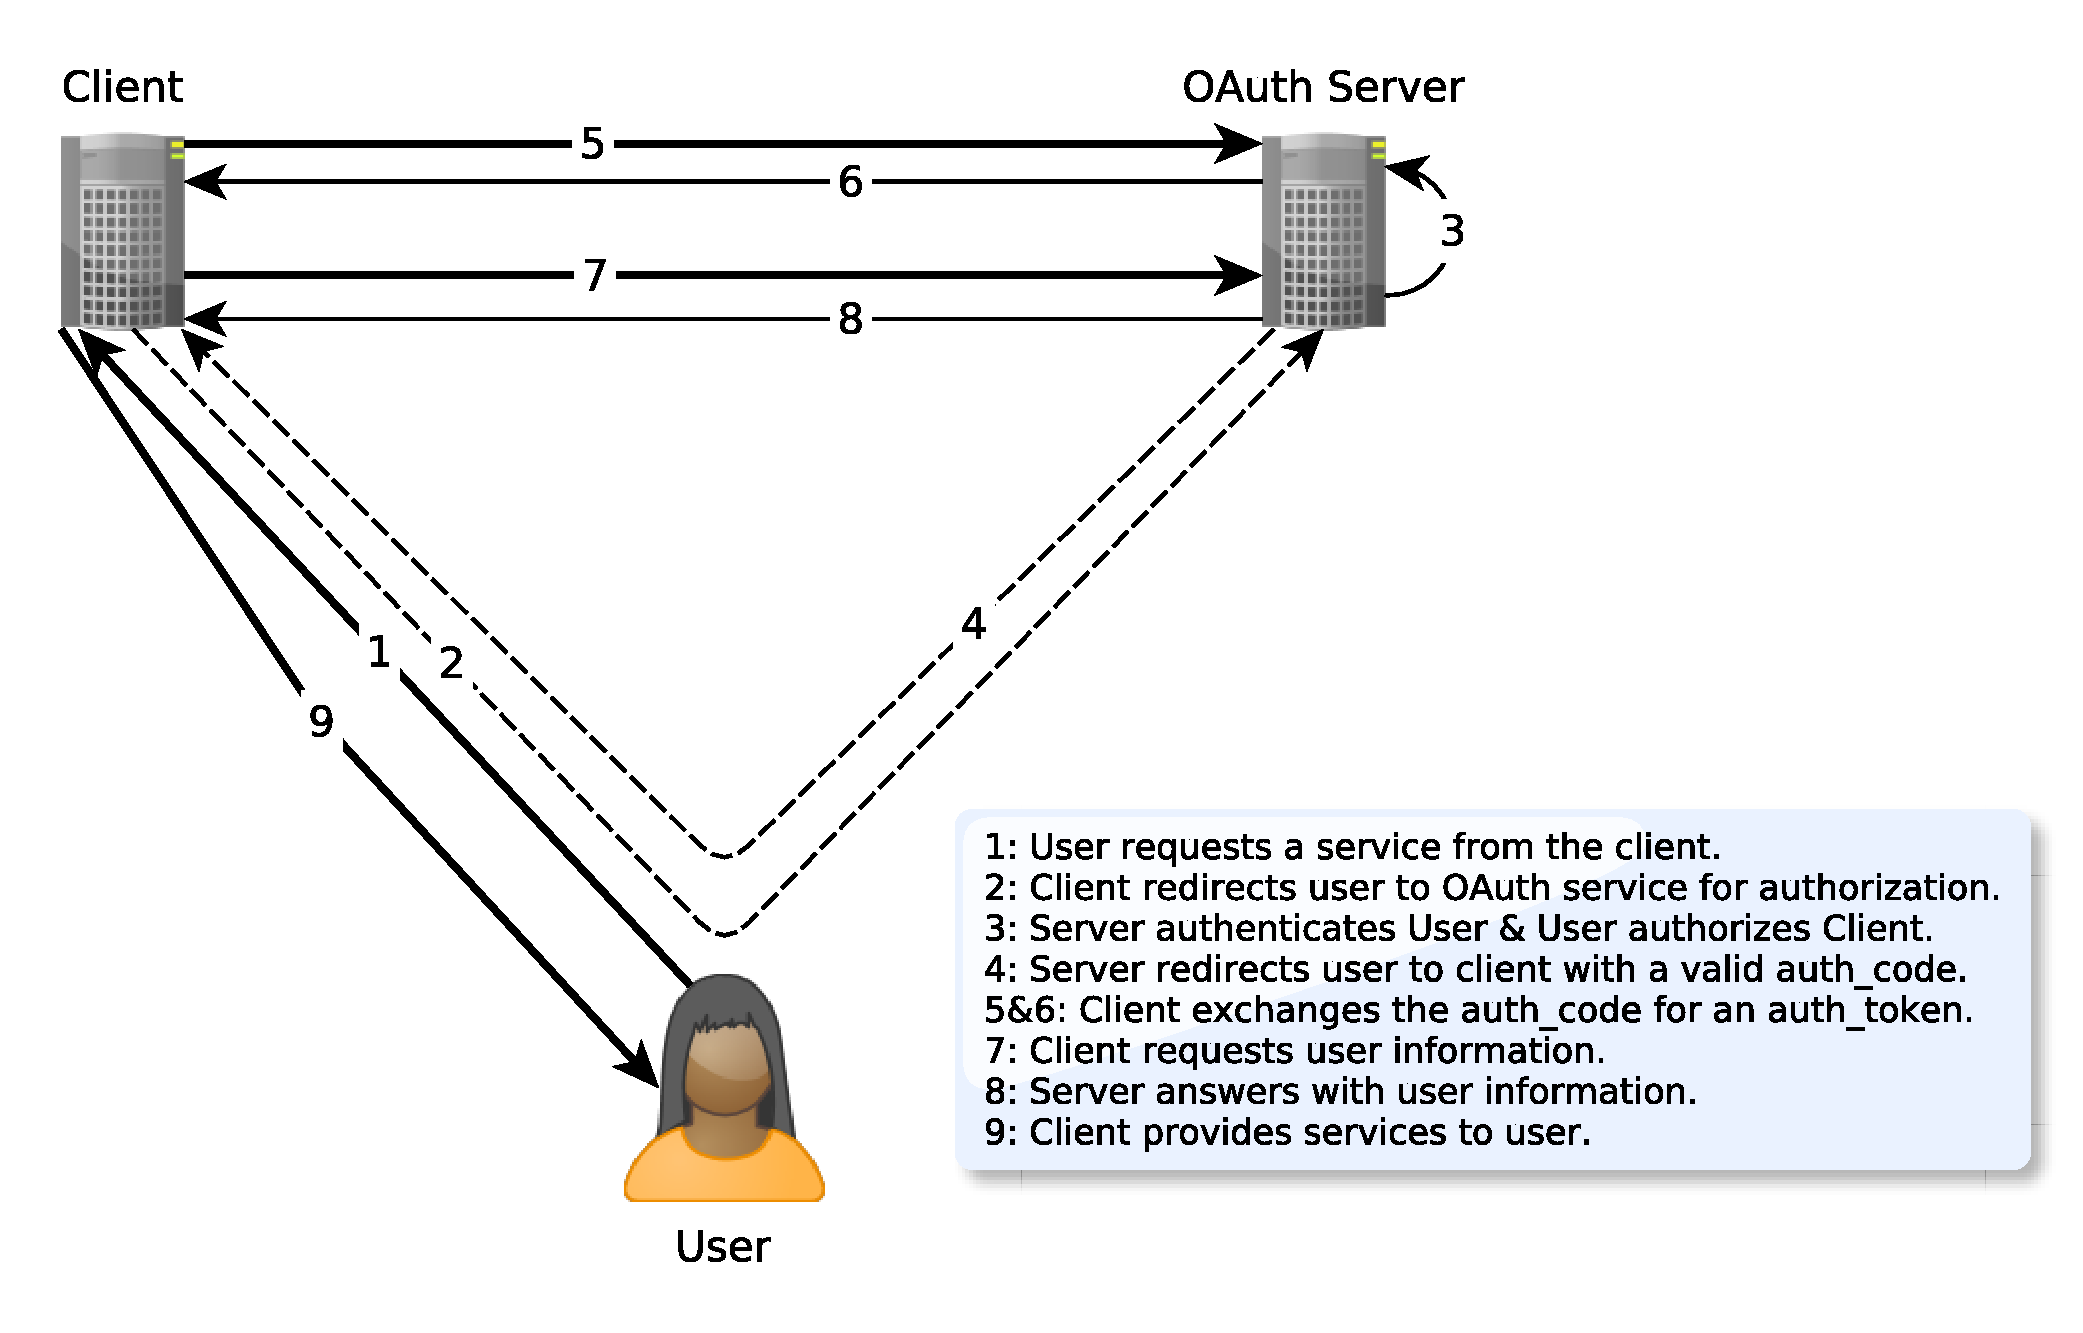
\includegraphics[width=15.5cm]{img/oauth2_workflow}
\caption{3-legged OAuth}
\label{pic:oauth2_workflow}
\end{figure}

Ein üblicher \emph{OAuth 2} Autorisierungsablauf, wie in Abbildung \ref{pic:oauth2_workflow} skizziert, wird durch einen Benutzer eingeleitet, der auf geschützte Dienste einer Client-Anwendung zugreifen möchte \circled{1}.
Der Benutzer wird auf die zur Client-Anwendung gehörige \emph{Autorisierungsseite} auf dem OAuth-Server weitergeleitet \circled{2}.
Dort muss er sich, falls noch nicht geschehen, authentifizieren und der Client-Anwendung Zugriffsrechte zugestehen \circled{3}.
Aus Transparenzgründen soll der OAuth-Server dem Benutzer \emph{vor} einer Autorisierung das beanspruchte Scope offenlegen.
Nach einer erfolgreichen Autorisierung wird der Benutzer auf eine, von der Client-Anwendung in \circled{2} festgelegten, Seite des Clients weitergeleitet \circled{4}.
Bei dieser Weiterleitung wird ein \emph{Authorization Code} als Variable im Request übergeben.
Diesen tauscht die Client-Anwendung beim OAuth-Server gegen ein \emph{Access Token} \circled{5} \& \circled{6}.
Nach einem erfolgreichen Token-Tausch hat der Benutzer gegenüber der Client-Anwendung bewiesen, dass er einen gültigen Account bei dem OAuth-Server besitzt.
Falls eine \emph{anonyme} Benutzung vorgesehen ist, kann die Client-Anwendung nach einem \emph{erfolgreichen} Token-Tausch mit \circled{9} fortfahren.
Mit dem \emph{Acces Token} kann die Client-Anwendung nun auf die Ressourcen des Benutzers zugreifen \circled{7} \& \circled{8}.
Letztendlich kann die Client-Anwendung dem Benutzer ihre Dienste zur Verfügung stellen \circled{9}.

\subsection{Sicherheit}
\label{sec:oauth/security}

Da es sich bei OAuth um eine Protokollspezifikation handelt, hängt die Sicherheit des Systems \emph{maßgeblich} von der jeweiligen Implementierung ab.
Mit \emph{OAuth 2} wurde, in einem eigenen \cite{RFC6750}, auch die Benutzung von \textbf{Bearer Tokens} vorgestellt.
Bearer Token sind eindeutige Zeichenketten die anstelle von \emph{Credentials} benutzt werden um auf Ressourcen zuzugreifen.
Authorization Codes, Authorization Tokens und Refresh Tokens können als Bearer Tokens realisiert werden.
Der Besitzt eines Bearer Token autorisiert den Zugriff auf die damit verbundenen Ressourcen.
Aus Sicherheitsgründen werden sie durch regelmäßige Invalidierung kurzlebig gehalten.
Durch ihre Kurzlebigkeit bringt der Besitz eines Tokens einem Angreifer nur kurzzeitig einen Vorteil.
Aus diesem Grund sind sie bei einer Authentifizierung statischem \emph{,,Wissen''}\footnote{vgl. \cite{WK06} Hannes Federrath, Andreas Pfitzmann: ,,IT-Sicherheit''. Kapitel 2.2 (S. 276-278)} vorzuziehen.
Bearer Token müssen bei \emph{jedem} Request übertragen werden und sind \emph{nicht} signiert, weshalb sämtliche Kommunikation \emph{zwingend} TLS verschlüsselt erfolgen muss.
Da \emph{OAuth 2} vorrangig auf TLS Verschlüsselung setzt, ist es maximal so sicher wie TLS selbst.

Im Juli 2012, kurz vor Fertigstellung der \emph{OAuth 2} Spezifikation, verkündete der Hauptautor Eran Hammer seinen Rücktritt.
Diesen begründet er vor allem mit einer geringeren Sicherheit gegenüber der Vorgängerversion.\footnote{vgl. Eran Hammer: OAuth 2.0 and the Road to Hell. \url{http://hueniverse.com/2012/07/oauth-2-0-and-the-road-to-hell/} (Zugriff am 01.03.2013)}
Hammer zufolge besteht das Kernproblem in einem unüberbrückbaren Konflikt zwischen der Web- und Konzern-Welten.
Trotz seiner Kritik räumt er ein, dass \emph{OAuth 2} \emph{,,in den Händen eines Entwicklers mit tiefgründigem Verständnis der Web-Sicherheit''} zu einer sicheren Implementierung führen kann.

% TODO http://homakov.blogspot.de/2013/03/oauth1-oauth2-oauth.html

\newpage
\section{OAuth InfRZ}
\label{sec:oauth-infrz}

\subsection{Anforderungen}
\label{sec:oauth-infrz/requirements}

Die Implementierung eines Single-Sign-On-Dienstes für den Fachbereich Informatik der Universität Hamburg muss \emph{sicher, vertrauenswürdig, benutzerfreundlich, selbsterklärend, wart- und erweiterbar} sein.
Neben den eben genannten Eigenschaften sollte eine \textbf{Client-Library} existieren.

\begin{quote}
\emph{,,What are the attributes of good software?\\
Good software should deliver the required functionality and performance to the user and should be maintainable, dependable, and usable.''}
\begin{flushright}
\small{-- \cite{Som10} Section 1.1}
\end{flushright}
\end{quote}

Die \textbf{Sicherheit von Webanwendungen} ist ein zentraler Faktor in der Webentwicklung.
Eine sichere Anwendung lässt keinen unautorisierten Zugriff auf ihre Daten zu.\footnote{vgl. \cite{Som10} Section 10.1.1}
Sie umfasst alle zur Laufzeit der Anwendung getroffenen Maßnahmen zur Einhaltung der \emph{Sicherheitsleitlinie}.
Eine Web-Anwendung ist \emph{hinreichend} sicher, wenn Maßnahmen gegen alle bekannten Angriffsszenarien getroffen wurden.
%TODO definition sicher ?

Eine \textbf{vertrauenswürdige Webanwendung} nutzt die Informationen eines Benutzers \emph{nicht} anders als von ihm erwartet und gewollt.
Als Authentifizierungs- und Autorisierungsdienst müssen Benutzer OAuth InfRZ zwingend sensible Credentials anvertrauen.
Mit der offenen Verfürbarkeit des Quellcodes werden die Prozesse einer Anwendung transparenter und somit vertrauenswürdiger.

%\footnote{vgl. Wikipedia: Webdesign. \url{http://de.wikipedia.org/wiki/Webdesign} (Zugriff am 03.03.2013)}
Eine \textbf{benutzerfreundliche Webanwendung} funktioniert intuitiv und bietet den Benutzern bekannte Elemente.
Benutzer haben in der Regel wenig Motivation sich mit komplizierten Prozessen zu beschäftigen, weshalb es wichtig ist Webanwendungen so benutzerfreundlich wie möglich zu gestalten.
Das \emph{Webdesign (Gestaltung, Aufbau und Nutzerführung)} entscheidet maßgeblich über die \emph{Benutzerfreundlichkeit (Usability)}.
Eine höhere Usability kann durch den Einsatz von verbreiteten Frameworks\footnote{vgl. \cite{Som10} Chapter 16} erzielt werden.

Bei \textbf{selbsterklärenden Webanwendungen} werden Benutzer stets über den Zweck der aktuell besuchten Seite informiert und es werden ihnen ihre Optionen aufgezeigt.
Selbsterklärende Webanwendungen sind benutzerfreundlicher und schaffen durch die dazugewonnene Transparenz Vertrauen.

Eine \textbf{wart- und erweiterbare  Webanwendung} lässt sich einfach an neue Anforderungen anpassen.
In Anbetracht der Tatsache, dass der Autor das Projekt mit der Fertigstellung an das Rechenzentrum übergibt, ist es umso wichtiger die Anwendung für andere Entwickler verständlich zu implementieren.
Eine hohe Wartbarkeit erreicht man unter anderem durch eine gute Dokumentation und eine sinnvolle Benutzung von verbreiteten Programmierparadigmen und Entwurfsmustern.\footnote{vgl. \cite{Som10} Section 6.3 \& Section 7.2}

Eine gut dokumentierte \emph{Client-Library} bietet Entwicklern eine leicht verständliche Schnittstelle für den Zugriff auf OAuth InfRZ.
Sie bietet eine fertige Implementierung aller Prozessabläufe, die durch Methodenaufrufe steuerbar sind.
Entwickler müssen sich dadurch nicht mehr mit den Spezifikationen des Authentifizierungsprozesses beschäftigen.
Eine \emph{Client-Library} sollte Informationen in wohlgeformten Datenstrukturen zurückliefern wodurch deren Verarbeitung vereinheitlicht und vereinfacht wird.
Die Client-Library muss gut dokumentiert und programmiersprachenunabhängig\footnote{damit Entwickler ihre Client-Anwendung in der Sprache ihrer Wahl schreiben können} implementierbar sein.

\subsection{Benutzung}
\label{sec:oauth-infrz/usage}

OAuth InfRZ läuft bereits auf einem Rechner des Rechenzentrums\footnote{erreichbar aus dem Informatik internen Netz unter \url{https://svs-sso.informatik.uni-hamburg.de}} und kann mithilfe der \textbf{Demo Anwendung}\footnote{erreichbar aus dem Informatik internen Netz unter \url{https://svs-sso.informatik.uni-hamburg.de/Demo}} ausprobiert werden.
Aus Gründen der Barrierefreiheit\footnote{vor allem in Rücksichtname auf unsere internationalen Studierenden} wird OAuth InfRZ in Englisch angeboten.
Übersetzungen in andere Sprachen lassen sich mit mittlerem Aufwand nachrüsten.
Die Oberfläche von OAuth InfRZ wurde möglichst schlicht gehalten.
Im folgenden wird auf die Benutzung und Oberfläche von OAuth InfRZ eingegangen.

\subsubsection{Benutzerrollen}

OAuth InfRZ wird von zwei Benutzerrollen benutzt, die unterschliedliche Rechte und Aufgaben besitzen.

\begin{description}
	\item[Benutzer] \hfill \\
		Mit \textbf{Benutzer} werden die Endnutzer bezeichnet.
		Sie benutzen OAuth InfRZ um sich gegenüber Anwendungen zu authentifizieren und diese mit dem Zugriff auf ihre Information zu autorisieren. 
		Sie haben Zugriff auf Haupt, Login-, und Autorisierungsseiten.
	\item[Client-Moderator] \hfill \\
		\textbf{Client-Moderatoren} verwalten Client-Anwendungen von OAuth InfRZ.
		Sie können Client-Anwendungen erzeugen, bearbeiten und löschen.
		Sie haben Zugriff auf die zum Ressourcen-Zugriff benötigten Credentials -- \emph{Client-ID} und \emph{Client-Secret}.
		Es ist ihre Aufgabe den Entwicklern ihrer Client-Anwendungen die dazugehörigen Credentials zur Verfügung zu stellen.
\end{description}

\subsubsection{Menüleiste}

Authentifizierte Benutzer werden namentlich begrüßt.
So wird sichergestellt, dass der Benutzer zu jedem Zeitpunkt weiß mit welchem Account er authentifiziert ist.
Client-Moderatoren wird der zusätzliche Menüpunkt \emph{,,Manage clients''} angezeigt, mit dem sie Zugriff auf das Client-Management-System erhalten.
Abbildung \ref{pic:oauth_infrz/navbar} zeigt eine vollständige Menüleiste.

\begin{figure}[h!]
\centering
\includegraphics[width=15cm]{img/oauth_infrz/navbar}
\caption{Menüleiste}
\label{pic:oauth_infrz/navbar}
\end{figure}

\subsubsection{Hauptseite}

Die in Abbildung \ref{pic:oauth_infrz/home} dargestellte Hauptseite bietet eine Erklärung der Funktionalität und fasst alle wichtigen Informationen über den Dienst zusammen.
Sie bietet Links zur verwendeten Lizenz, technischen Dokumentation und zum Repository des Quellcodes.
Diese Maßnahmen sollen die Verstrauenswürdigkeit fördern.

\begin{figure}[h!]
\centering
\includegraphics[width=15cm]{img/oauth_infrz/home}
\caption{Hauptseite}
\label{pic:oauth_infrz/home}
\end{figure}

\subsubsection{Authentifizierung}

Benutzer können sich auf der \textbf{Loginseite} gegen das Active Directory authentifizieren.
Die Eingabefelder der Loginseite sind selbsterklärend.
Üblicherweise gelangen Benutzer über die Autorisierungsanfrage eines Clients auf die Loginseite.
In diesen Fällen wird, wie in Abbildung \ref{pic:oauth_infrz/login_client} illustriert, eine farblich hervorgehobene Info-Box eingeblendet in welcher der Client genannt wird.
Außerdem wird der Benutzer nach einer erfolgreichen Authentifizierung zur zum Client gehörigen Autorisierungsseite weitergeleitet.

\begin{figure}[h!]
\centering
\includegraphics[width=15cm]{img/oauth_infrz/login_client}
\caption{Loginseite: Authentifizierungsaufforderung von ,,Demo Application''}
\label{pic:oauth_infrz/login_client}
\end{figure}

\subsubsection{Autorisierung}

Um einen Client-Dienst zu nutzen, müssen Benutzer diesen erst autorisieren.
Dies geschieht über die in Abbildung \ref{pic:oauth_infrz/authorize} gezeigte \textbf{Autorisierungsseite} des Clients.
Der Benutzer legt dabei fest, auf welche seiner Informationen die Client-Anwendung über OAuth InfRZ zugreifen darf.
Diese Seite stellt Informationen zur Client-Anwendung und dem angeforderten Scope bereit.
Ein Client-Moderator legt das von einer Client-Anwendung angeforderte Scope fest.
Dabei kann der Client-Moderator sowohl erforderliche (required) als auch optionale Zugriffsrechte beantragen.
\textbf{Optionale Felder} können Benutzer abwählen und dem Client somit den Zugriff auf die dazugehörige Ressource verwehren.
\textbf{Erforderliche Felder} hingegen werden ausgegraut angezeigt und können nicht abgewählt werden.
Nach einer erfolgreichen Autorisierung wird der Benutzer zu einer vom Client bestimmten URL des Clients weitergeleitet.

\begin{figure}[h!]
\centering
\includegraphics[width=15cm]{img/oauth_infrz/authorize}
\caption{Autorisierungsseite für ,,Demo Application''}
\label{pic:oauth_infrz/authorize}
\end{figure}

\subsubsection{Client-Management}

Das \textbf{Client-Management} ist ausschließlich für Client-Moderatoren einsehbar.
Clients können von einem Client-Moderator angelegt und verwaltet werden.
Technisch sind Moderatoren Benutzer mit besonderen Rechten.
Für die Benutzung des Client-Managements wird eine funktionierende JavaScript-Engine benötigt.
Client-Moderatoren sollen im laufenden Betrieb vom Rechenzentrum verwaltet werden.\footnote{eine ausführliche Diskussion zu diesem Thema gibt es in Abschnitt \ref{sec:oauth-infrz/moderator}}


\begin{figure}[h!]
\centering
\includegraphics[width=15cm]{img/oauth_infrz/clients_overview}
\caption{Client-Übersichtsseite}
\label{pic:oauth_infrz/clients_overview}
\end{figure}

Über den Menüpunkt \emph{,,Manage clients''} gelangt ein Moderator auf die in Abbildung \ref{pic:oauth_infrz/clients_overview} illustrierte \emph{Client-Übersichtsseite}.
Auf dieser Seite werden alle vom Moderator verwalteten Clients aufgelistet.
Von hier aus gelangt man über den \emph{,,Register a new client''}-Button zur in Abbildung \ref{pic:oauth_infrz/client_new} gezeigten \textbf{Client-Registrierungsseite}.
Die Namen in der Tabelle sind Links zur entsprechenden \textbf{Clientseite} (Abbildung \ref{pic:oauth_infrz/client}).

\begin{figure}[h!]
\centering
\includegraphics[width=15cm]{img/oauth_infrz/client_new}
\caption{Client-Registrierungsseite}
\label{pic:oauth_infrz/client_new}
\end{figure}

Auf der \textbf{Client-Registrierungsseite} können neue Clients bei OAuth InfRZ registriert werden.
Die Client-Registrierungsseite bietet ein HTML-Formular zur Einstellung der Client Eigenschaften.
Nicht sofort ersichtliche Felder werden mit \textbf{Tooltips}\footnote{vgl. TechTerms: Tooltip. \url{http://www.techterms.com/definition/tooltip} (Zugriff am 15.03.2013)} erklärt.
Der \textbf{,,Name''} soll für den Dienst der dazugehörigen Webanwendung \emph{passend} gewählt werden.
Am besten entspricht er dem in der Webanwendung selbst benutzten Namen.
Aus der \textbf{Beschreibung (,,Description'')} soll ersichtlich sein, was dieser Dienst macht \emph{und} weshalb er eine Autorisierung vom Benutzers erfordert.
Als \textbf{,,Host''} ist der \emph{Hostname} oder die \emph{IP-Adresse} des Dienstes einzutragen.
Eine Zugriffsbeschränkung der Requests über die Adresse des Client Servers wird in Abschnitt \ref{sec:oauth-infrz/host} diskutiert.
Als \textbf{,,Redirect URI''} ist die zur Verarbeitung des Authorization Codes vorgesehene Seite der Client-Anwendung anzugeben.
Felder zu nicht als \emph{verfügbar (,,available'')} markierten \textbf{,,Scopes''} sind deaktiviert und werden ausgegraut dargestellt.
Die \textbf{,,Scope info''} wird auf der Autorisierungsseite als Erklärung zum Scope angezeigt.
Sie soll Auskunft darüber geben, weshalb der Dienst Zugriff auf diese Information benötigt.

\begin{figure}[h!]
\centering
\includegraphics[width=15cm]{img/oauth_infrz/client}
\caption{Clientseite}
\label{pic:oauth_infrz/client}
\end{figure}

Neben einer Auflistung aller einstellbaren Eigenschaften, beinhalten Clientseiten die Credentials \emph{(die ,,Client-ID'' und das ,,Client-Secret'')}. Bei beiden Werten handelt es sich um eine zufällige Zeichenkette.

\begin{description}
	\item[Client-ID] \hfill \\
		Jeder Client besitzt eine eindeutige \textbf{Client-ID} anhand der er bei OAuth InfRZ identifiziert wird.
	\item[Client-Secret] \hfill \\
		Das \textbf{Client-Secret} ist ein Geheimins, durch dessen Angabe sich ein Client gegenüber OAuth InfRZ authentifiziert.
		Die Betreiber einer Client Anwendung müssen es angemessen vor unbefugtem Zugriff schützen.
\end{description}

Clientseiten bieten die Optionen den Client zu löschen, zu editieren und sich neue Credentials zuweisen zu lassen.
Vor dem Löschen eines Clients wird eine Löschbestätigung angezeigt.
Die Oberfläche zum Bearbeiten des Clients ähnelt der Client-Registrierungsseite.

\subsection{Eingesetzte Werkzeuge}
\label{sec:oauth-infrz/used-tools}

Als \textbf{Werkzeuge} werden in diesem Abschnitt alle zur technischen Umsetzung benutzten Programme, Programmiersprachen und Frameworks bezeichnet.
Alle eingesetzten Werkzeuge müssen den Entwickler dabei unterstützen die an die Anwendung gestellten Anforderungen umzusetzen.
Grundsätzlich gilt es für das Anwendungsgebiet angemessene Werkzeuge einzusetzen.
Werkzeuge sind angemessen, wenn sie eine saubere, hinreichend perfomante Lösung für das vorgesehene Anwedungsgebiet ermöglichen.
Um eine unnötige Komplexität zu verhindern, gilt es vor dem Einsatz einer neuen Technologie gründlich abzuwägen, ob ihr Nutzen den damit zusammenhängenden Mehraufwand rechtfertigt.

\subsubsection{Back-End: PHP 5.4, SQLite, nginx}
\label{sec:oauth-infrz/back-end}

Zum \textbf{Back-End} gehören in der Webentwicklung alle Prozesse, die \emph{serverseitig} ausgeführt werden.

% PHP
\textbf{PHP: Hypertext Preprocessor (PHP)} ist eine \emph{serverseitig ausgeführte Skriptsprache}.
Es ist die verbreitetste\footnote{vgl. w3techs: Usage of server-side programming languages for websites. \url{http://w3techs.com/technologies/overview/programming_language/all} (Zugriff am 04.03.2013)} Programmiersprache für Webanwendungen.
PHP ist imperativ, objektorientiert und frei.
PHP erschien erstmals 1995, seither wurde es stetig korrigiert, erweitert und verbessert.
Die \emph{PHP-Syntax} ist an verbreitete Programmiersprachen wie C, C++, Java oder Perl angelehnt, weshalb PHP für erfahrene Entwickler leicht erlernbar ist.
Zusätzlich zu zahlreichen \emph{PHP-Libraries}\footnote{vgl. Wikipedia: List of PHP libraries. \url{http://en.wikipedia.org/wiki/List_of_PHP_libraries} (Zugriff am 04.03.2013)} liefert  das WWW eine Vielzahl von Erweiterungen, Anleitungen und Beispielen, die Entwickler unterstützen.
Seit \emph{PHP 5.3} liegt der Fokus primär auf der \emph{Objektorientierung}\footnote{vgl. Heise Developer: PHP 5.3 mit vielen neuen Funktionen. \url{http://www.heise.de/developer/meldung/PHP-5-3-mit-vielen-neuen-Funktionen-187509.html} (Zugriff am 04.03.2013)}, welche eine moderne und saubere Programmierung ermöglicht.
PHP-Entwickler schätzen die schwache, dynamische Typisierung, die eine agile Entwicklung unterstützt.
Auf \emph{\url{http://php.net}} befindet sich eine ausführliche Dokumentation mit Beispielen und Benutzer-Kommentaren.

Aufgrund einer großen Community und der damit einhergehenden Erfahrung sollte PHP bei der Entwicklung von Webanwendungen in Erwägung gezogen werden.
PHP liefert Libraries für alle Kernfunktionalitäten von OAuth InfRZ, weshalb es sich zur Benutzung eignet.

% SQLite
\textbf{SQLite} ist ein \emph{relationales Datanbanksystem}.
Als eingebettetes Datenbanksystem\footnote{vgl. SQLite: Most Widely Deployed SQL Database. http://www.sqlite.org/mostdeployed.html (Zugriff am 04.03.2013)} ist der Anwendungsbereich von SQLite nicht auf Server begrenzt, vielmehr findet man es in den Programmen von zahlreichen Endgeräten.
SQLite ist public domain und unterstützt einen Großteil des in \cite{SQL1992} spezifizierten \emph{SQL92-Standard}.
Anstatt seine Informationen auf mehrere Dateien zu verteilen, speichert SQLite die komplette Datenbank in einer Datei, was die Komplexität verringert und eine Datensicherung vereinfacht.
SQLite zeichnet eine einfache Handhabung und geringe Größe\footnote{je nach Betriebssystem zwischen etwa 250 und 300 KiB} aus.
Die Wahl des Datenbanksystems ist maßgeblich von dem Einsatzszenario abhängig. Bei einer Webanwendung mit verschwindend geringer Last \emph{und} überschaubaren Datenmengen, wie OAuth InfRZ, ist SQLite eine gute Wahl.

% nginx
\textbf{nginx} ist ein freier \emph{high-performance Webserver}.
Er wird für seine hohe Performance, gute Skalierbarkeit, simple Konfiguration und Ressourcen-Sparsamkeit geschätzt und findet zunehmend Anwendung.\footnote{vgl. \cite{Ree08} Abstract}
Obwohl nginx den Anspruch hat sich auf die wesentlichen Funktionen eines Webservers zu beschränken, bietet es Administratoren alle wichtigen Konfigurations-, Debugging- und Maintenanceeigenschaften.

\subsubsection{Front-End: HTML5, CSS3, JavaScript}

Mit \textbf{Front-End} werden alle beim Nutzer angezeigten Ausgaben bezeichnet. Es bildet das Gegenstück zum \emph{Back-End}. 

% HTML
Die \textbf{Hypertext Markup Language (HTML)} ist die meistverwendete \emph{Auszeichnungssprache} im WWW.
Mit HTML werden die Elemente einer Webseite definiert und in einen Gesamtkontext gebracht.
Seit dem im November 1995 erschienenen \cite{RFC1866} hat sich HTML stetig weiterentwickelt und prägt Look and Feel des WWW maßgeblich.

% CSS
\textbf{Cascading Style Sheets (CSS)} ist eine \emph{Auszeichnungssprache}.
Sie werden überwiegend als Stilvorlagen für HTML und andere XML-Dokumente verwendet.
Im Gegensatz zu HTML wird CSS ausschließlich für die Gestaltung verwendet.
CSS erlaubt dem Entwickler das Erscheinungsbild vom Inhalt zu trennen.
Es existieren zahlreiche CSS-Frameworks die einem Entwickler bei der Implementierung des Designs unterstützen.

% JavaScript
\textbf{JavaScript (JS)} ist eine weit verbreitete, dynamisch typisierte und objektorientierte \emph{Skriptsprache}.
Ursprünglich wurde JS entwickelt um clientseitig im Webbrowser ausgeführt zu werden.
Es wird hauptsächlich verwendet um Webanwendungen dynamisch zu gestalten und das \textbf{Document Object Model (DOM)} zu manipulieren.
Heutzutage findet JS in weiteren Anwendungsgebieten\footnote{zum Beispiel als Programmiersprache für Webanwendungen mit dem Framework Node.js} Verwendung.
Bis zur Erscheinung von \emph{V8}, einer freien von Google entwickelten \emph{JS-Engine}, im September 2008 wurde JS zur Laufzeit interpretiert.
Durch den Einsatz von \emph{just-in-time} Kompilierung\footnote{just-in-time-Kompilierer übersetzen Programme zur Laufzeit in Maschinencode} erzielte V8 deutlich überlegene Ausführungszeiten\footnote{vgl. Heise Online: Google Chrome überholt die Konkurrenz. \url{http://www.heise.de/newsticker/meldung/Google-Chrome-ueberholt-die-Konkurrenz-202963.html} (Zugriff am 04.03.2013)} als alle bis dato verwendeten JS-Engines.
Mittlerweile haben auch andere Browser auf \emph{just-in-time} Kompilierung umgestellt.

Die Kombination aus HTML5, CSS3 und JavaScript hat mit der Nachfrage an plattformunabhängigen Programmiermöglichkeiten\footnote{besonders im Smart Phone Sektor} an Bedeutung gewonnen.
Eine moderne Webanwendung ohne diese Sprachen zu programmieren ist undenkbar.

\subsubsection{Frameworks: Twig, Bootstrap, jQuery}

% Frameworks
\textbf{Frameworks} sind leicht erweiterbare \emph{Programmiergerüste}.
Sie unterstützen Softwareentwicklung durch ein Angebot an erprobter Funktionalität.
Der Einsatz von verbreiteten Frameworks trägt zu einer besseren Wartbarkeit bei.\footnote{vgl. \cite{Som10} Chapter 16}

% Twig
\textbf{Twig} ist eine Open Source \emph{template engine für PHP}.
Mit Twig lassen sich statische HTML-Seiten aus \emph{dynamischen} Twig-Dateien kompilieren.
In \emph{Twig-Dateien} kann man -- zusätzlich zu HTML -- Kontrollstrukturen, Variablen und Funktionen benutzen um den Inhalt dynamisch anzupassen.
Die Einführung von Vererbungsfunktionalität reduziert Codeduplikation und struktuiert den Code durch Kapselung.
Der Einsatz von Twig macht das Frontend wartbarer und leichter verständlich.

% Bootstrap
\textbf{Bootstrap} ist ein freies, von Twitter geschaffenes \emph{CSS Framework}.
Bootstrap bietet eine große Auswahl an \emph{Web-Komponenten} für die Benutzeroberfläche.
Diese sind aufgrund steigender Beliebtheit vielen Benutzern schon bekannt was eine bessere Usability zu Folge hat.

% jQuery
\textbf{jQuery} ist das meistverwendete\footnote{w3techs: Usage of JavaScript libraries for websites. \url{http://w3techs.com/technologies/overview/javascript_library/all} (Zugriff am 05.03.2013)} \emph{JavaScript Framework}.
jQuery bietet eine große Auswahl an Funktionen mit deren Hilfe man auf DOM-Objekte zugreifen und manipulieren kann.
jQuery ist ein Free Software Projekt.

Zu diesen drei Frameworks gibt es ausführliche Dokumentationen mit Code-Beispielen und eine hilfreiche Community.

\subsubsection{Verschlüsselung: TLS}
\label{sec:oauth-infrz/tls}

Bei der Übertragung von Credentials ist es erforderlich eine angemessene Verschlüsselung zu wählen.
Trotz der in Abschnitt \ref{sec:basics-security} angesprochenen Sicherheitsmängel ist TLS aufgrund seiner weiten Verbreitung zu wählen.
Es ist zu erwarten, dass Browser die sicherere Version \emph{TLS 1.2} in naher Zukunft unterstützen werden.

\textbf{OpenSSL} ist eine freie Sammlung von \emph{SSL und TLS tools} für den Server.
Mit OpenSSL können Verbindungen mit TLS verschlüsselt werden.

% TODO Software ?
%\subsubsection{Software}

%Im Folgenden wird eine Auswahl der zur Entwicklung und Betreibung von \emph{OAuth %InfRZ} verwendeten Software geboten.
%\textbf{\emph{PHPStorm}} ist eine proprietäre Entwicklungsumbebung für \emph{PHP}.
%\textbf{\emph{Ubuntu}} ist ein freies Betriebssystem und wird auf dem Server eingesetzt.

\subsection{Eingesetzte Konzepte}
\label{sec:oauth-infrz/concepts}

Mit eingesetzten \textbf{Konzepten} werden in diesem Abschnitt Programmierparadigmen, Entwurfsmuster und Architekturmuster bezeichnet.
Sie dienen der Strukturierung von Code und machen diesen somit wartbarer und leichter verständlich.
Für sie gelten analoge Anforderungen wie für Werkzeuge\footnote{in der Einleitung zu Abschnitt \ref{sec:oauth-infrz/used-tools} beschrieben}.

% OOP - Objektorientierte Programmierung
\textbf{Objektorientierte Programmierung (OOP)} ist ein weit verbreitetes \emph{Programmierparadigma}.
Es beruht auf der Philosopie der Objektorientierung, nach der Teile des Codes ihrem Zweck nach in Klassen geteilt werden.
Klassen bilden ein abstraktes Konstrukt und somit Blaupausen für Objekte. Sie beschreiben Funktionen ihrer zugehörigen Objekte.
Objekte sind Instanzen von Klassen, die mit anderen Objekten kommunizieren und interagieren.
\emph{,,The class holds the shared behavior for its instances''}\footnote{vgl. \cite{Kay93} IV.}.
Objektorientierte Programmierung schafft\footnote{im Vergleich zur klassischen prozedualen Programmierung} klare Strukturen und macht den Quellcode dadurch wartbarer und leichter verständlich.

% MVC - Model View Controller
\textbf{Model View Controller (MVC)} ist ein \emph{Entwurfsmuster} zur Gliederung von Code nach seiner Aufgabe.
Grundkonzept von MVC ist es durch die Aufteilung der Softwareteile nach dem \textbf{Datenmodell (Model)}, der \textbf{Benutzerausgabe (View)} und der \textbf{Programmsteuerung (Controller)} eine bessere Modularität zu erzielen.\footnote{vgl. \cite{Som10} Section 6.3}
Durch den Einsatz von MVC gewinnt Code an Struktur und es wird leichter Teile des Codes auszutauschen.
Durch den Einsatz von MVC wird eine Anwendung wartbarer und leichter verständlich.

% Front-Controller
\textbf{Front-Controller} ist ein \emph{Architekturmuster} mit dessen Hilfe sich Adressen auf Controller abbilden lassen.
Front-Controller bieten einen zentralen Einstiegspunkt in eine Webanwendung.
Alle eingehenden Requests werden zunächst von dem \emph{Front-Controller} bearbeitet.
Dieser wählt den zum Request passenden Controller und startet diesen.
Front-Controller strukturieren Code und machen ihn übersichtlicher.
Dadurch wird Code wartbarer und leichter verständlich.

% Autoloader
\textbf{Autoloader} laden benötigte Klassen automatisch nach.
Anstatt die vollständige Anwendung zur Initialisierung zu laden, wird bei dem Einsatz eines Autoloaders nur ein minimaler Kern geladen.
Durch den Einsatz von Autoloadern werden Anwendungen performanter, da unbenutzte Teile der Anwendung nicht geladen werden.

\subsection{Technische Realisierung}

\subsubsection{Versionierung}

% Git
\textbf{Git} ist ein freies \emph{verteiltes Versionierungssystem}.
Ein Versionierungssystem dokumentiert die Veränderungen von Dokumenten.
Ein verteiltes Versionierungssystem benötigt keinen zentralen Server, da es dezentral laufen kann.
Das \emph{Git-Repository} von OAuth InfRZ wird auf \emph{GitHub}\footnote{vgl. OAuth InfRZ. \url{https://github.com/Senci/oauth-infrz} (Zugriff am 14.03.2013)} weltöffentlich zur Verfügung gestellt.

\subsubsection{Verzeichnisstruktur und Dateien}

Die \textbf{Verzeichnisstruktur} von OAuth InfRZ wird maßgeblich vom \emph{MVC-Pattern} bestimmt.
Im Folgenden wird auf die einzelnen Verzeichnisse und die darin enthaltenden Dateien eingegangen um einen Kontext dieser Dateien zur Anwendung aufzubauen.

Im Hauptverzeichnis befinden sich die Lizenzinformation (\emph{COPYING}), eine technischen Dokumentation (\emph{README.md}), die Konfigurationsdatei (\emph{config.ini}) und der zentrale Einstiegspukt (\emph{index.php}) in die Anwendung.
In der \emph{index.php} werden einige globale Einstellungen getroffen, die Session initialisiert, die Konfiguration geladen und der Front-Controller gestartet.

Das Verzeichnis \textbf{Control} enthält neben den eigentlichen Controllern in dem Unterverzeichnis \textbf{Modules} auch den Autoloader (\emph{Autoloader.php}) und den Front-Controller (\emph{FrontController.php}).
Im Unterverzeichnis \textbf{Security} befindet sich das Auth-Factory-Interface (\emph{AuthFactoryInterface.php}) und die LDAP-Auth-Factory (\emph{LDAPAuthFactory}).
Implementierungen des Auth-Factory-Interfaces können genutzt werden um den Authentfizierungs-Mechanismus auszutauschen.
Dadurch ist OAuth InfRZ mit wenig Aufwand an eine veränderte Infrastruktur anpassbar.
Die LDAP-Auth-Factory ist eine Implementierung des Auth-Factory-Interfaces.

Das Verzeichnis \textbf{Model} enthält das Datenmodell (jede Klasse in einer eigenen PHP-Datei) und den Database-Wrapper (\emph{DatabaseWrapper.php}).
Der Database-Wrapper stellt Funktionen für den Zugriff und die Manipulation der Datenbank zur Verfügung.
Jeglicher Zugriff und Manipulation der Datenbank soll über den Database-Wrapper geschehen.

Das Verzeichnis \textbf{View} enthält die \emph{twig Templates} (jedes Template in einer eigenen twig-Datei) und den Response-Builder (\emph{ResponseBuilder.php}).
Der Response-Builder ist für alle Ausgaben zuständig.
Er stellt Funktionen zur Generierung und Rückgabe von Antworten bereit.

Das Verzeichnis \textbf{Client} enthält die \emph{Client-Library}. Genauere Informationen zur Client-Library gibt es in Abschnitt \ref{sec:oauth-infrz/client}.

Das Verzeichnis \textbf{Demo} enthält eine simple \emph{Client-Anwendung} die zur Demonstration der Funktionalität und Veranschaulichung des Autorisierungsablaufs von OAuth InfRZ dient.

Das \textbf{Resources} Verzeichnis enthält alle vom Browser für die Anzeige benötigten Ressourcen. Dazu gehören CSS-Stylesheets (im Unterverzeichnis \textbf{css}), JS-Skripte (im Unterverzeichnis \textbf{js}) und Bilder (im Unterverzeichnis \textbf{img}). Im Unterverzeichnis \textbf{bootstrap} befindet sich das Bootstrap Framework.

\subsubsection{Front-Controller}

Wie schon in Abschnitt \ref{sec:oauth-infrz/concepts} beschrieben dient ein \textbf{Front-Controller} dem Abbilden von Adressen auf Controller.
Durch den Einsatz eines Front-Controllers sind Entwickler nicht mehr dazu gezwungen ihre Verzeichnisstruktur nach den URLs zu modellieren.
Alle verfügbaren \textbf{Aktionen (Actions)} werden im Controller als Methoden deklariert.
Bei OAuth InfRZ erkennt nginx die eingehenden Requests nach ihrer URL und bildet diese -- sofern sie auf einen der eingetragenen regulären Ausdrücke passt -- auf den Front-Controller ab.
Informationen über den zuständigen Controller und die aufzurufende Action werden dabei intern in dem Feld \emph{,,action''} mit der Syntax \emph{,,Controller\_Action''} übertragen.
Intern funktioniert das über einen Redirect, der Benutzer bekommt davon allerdings nichts mit.
Der Front-Controller dekodiert das \emph{,,action''}-Feld, erstellt dynamisch eine Instanz des entsprechenden Controllers und ruft die entsprechende Action an dem Controller auf.
Bei PHP bietet es sich an zu diesem Zweck \textbf{variable Variablen}\footnote{vgl. PHP: Variable variables. \url{http://www.php.net/manual/en/language.variables.variable.php} (Zugriff am 14.03.2013)} zu benutzen.
Durch variable Variablen lassen sich die tatsächlich aufgerufenen Klassen und Methoden dynamisch zur Laufzeit bestimmen.
In Listing \ref{lst:variable} (Zeile 17 und 20) wird die Benutzung von variablen Variablen exemplarisch gezeigt.
Listing \ref{lst:variable} beinhaltet eine aus redaktionellen Gründen vereinfachte Version der \code{execAction} Methode des Front-Controllers.

\begin{minipage}{\textwidth}
	\lstinputlisting[name=VariableVariable,label=lst:variable,
	caption={Benutzung von variablen Variablen am Beispiel des Front-Controllers},
	style=PHP]
	{listings/front_controller.php}
\end{minipage}

\subsubsection{Auth-Factory}

Eine \textbf{Auth-Factory} ist eine Hilfsklasse für die Authentifizierung.
Die LDAP-Auth-Factory bietet eine Implementation des Auth-Factory-Interface für die LDAP-Authentifizierung am Informatik Rechenzentrum.
Sie nutzt die vom Benutzer zur Verfügung gestellten Credentials um auf einen Teil der im Active Directory gespeicherten Informationen zuzugreifen und bildet somit die Kernfunktionalität von OAuth InfRZ.
Diese Daten werden nach ihrem Zugriff aufbereitet und als \emph{,,User''}-Objekt zurückgegeben.
Die LDAP-Auth-Factory benutzt die von PHP zur Verfügung gestellte \emph{LDAP-Library} um mit dem Active Directory zu kommunizieren.
Listing \ref{lst:ldap} zeigt eine aus redaktionellen Gründen vereinfachte Version der \code{signIn} Methode.

\begin{minipage}{\textwidth}
	\lstinputlisting[name=ldap,label=lst:ldap,
	caption={LDAP-Authentifizierung mit der LDAP-Library von PHP},
	style=PHP]
	{listings/ldap.php}
\end{minipage}


\subsubsection{Sicherheit}
\label{sec:oauth-infrz/security}

TLS verschlüsselte Verbindungen erschweren \textbf{Man-in-the-middle}-Angriffe\footnote{vgl. \cite[Section 10.8]{RFC6749}}.

Bei Man-in-the-middle-Angriffen übernimmt ein Angreifer die Kommunikation zwischen Systemen, indem er sie abfängt und weiterleitet.
Dabei kann er die übermittelten Pakete lesen und modifizieren.
Eine solcher Angriff geschieht bei TLS auf den Schlüsselaustausch, um die Pakete entschlüsseln zu können.
Ein Angreifer gibt sich dabei jeweils als einer der Kommunikationspartner aus.\footnote{vgl. \cite[Section 8.7.2]{TW10}}
Die verschlüsselt übertragenen Pakete kann ein Angreifer nicht verwerten.
Zusätzliche Schutzmechanismen erschweren zudem eine Manipulation der  Kommunikation.
Alle erforderlichen Einstellungen werden in der Konfigurationsdatei der Server-Software getroffen.
Ein gültiges Zertifikat kann im Rechenzentrum beantragt werden.

\textbf{PHP Data Objects (PDO)} verringern die Anfälligkeit für \textbf{SQL-Injections}.
Als \emph{Abstraktionsschicht} für den Datenbankzugriff erlaubt PDO eine von der Wahl der Datenbank unabhängige Programmierung.
Eine \textbf{SQL-Injection} ist die Ausführung von unerwünschten \emph{SQL-Statements}, die ein Eingreifer in seine Eingaben einschleust.
Es werden Zeichen mit besonderer Bedeutung im SQL-Kontext verwendet um eine Anweisung einzuschleusen.
Die Verwendung von \textbf{Prepared Statements} trennt SQL-Befehle von den dazugehörigen Werten, welche beim Binden automatisch \emph{,,escaped''}\footnote{Zeichen mit besonderer Bedeutung werden in eine Escape-Sequenz umgewandelt} werden.
Durch konsequenten Einsatz von Prepared Statements kann die Anfälligkeit für SQL-Injections minimiert werden.
Listing \ref{lst:pdo} verdeutlicht exemplarisch die Benutzung von Prepared Statements.

\begin{minipage}{\textwidth}
	\lstinputlisting[name=pdo,label=lst:pdo,
	caption={Benutzung von Prepared Statements mit PHP Data Objects},
	style=PHP]
	{listings/prepared_statement.php}
\end{minipage}

An \textbf{Page-Token} gebundene Aktionen verhindern \textbf{Cross-site request forgery (CSRF)}.
Bei CSRF-Angriffen bringt ein Angreifer den Browser seines Opfers dazu Requests auszuführen.
Der Angreifer nutzt dabei offene Sessions des Opfers um Aktionen bei anderen Webanwendungen auszuführen.
Ein CSRF-Angriff kann ohne die Kenntnisnahme des Opfers durchgeführt werden.
Ein Page-Token ist ein an \emph{einen} Benutzer gebundenes Geheimnis.
Es wird üblicherweise als \emph{Hidden Field} in das \emph{HTML-Formular} eingefügt.
Für einen Angreifer ist es schwierig Page-Token auszulesen.
Da für jede Aktion ein gültiges Page-Token notwendig ist, verhindert deren Benutzung CSRF-Angriffe.
Bei OAuth InfRZ sind die Page-Tokens als Bearer Tokens realisiert und werden als \emph{Form-Encoded Body Parameter}\footnote{vgl. \cite[Section 2.2]{RFC6750}} übertragen.
Zur Erzeugung wird eine zufällige und eindeutige Zeichenfolge geschaffen, an den Benutzer gebunden und in die Datenbank eingefügt.
Listing \ref{lst:page_token_creation} beinhaltet eine vereinfachte Version des zuur Erzeugung eines Page-Token benutzten Codes.

\begin{minipage}{\textwidth}
	\lstinputlisting[name=page_token_creation,label=lst:page_token_creation,
	caption={Erzeugung eines Page-Token},
	style=PHP]
	{listings/page_token_creation.php}
\end{minipage} 

Bei der Verifizierung eines Page-Token wird die Benutzerzugehörigkeit und die zeitliche Gültigkeit des Tokens überprüft.
Ein Page-Token muss zum aktuell angemeldeten Benutzer gehören und darf nicht älter sein als 30 Minuten.
Listing \ref{lst:page_token_creation} zeigt eine vereinfachte Form des Codes mit dem ein Page-Token Verifiziert wird.

\begin{minipage}{\textwidth}
	\lstinputlisting[name=page_token_validation,label=lst:page_token_validation,
	caption={Verifizierung eines Page-Token},
	style=PHP]
	{listings/page_token_validation.php}
\end{minipage}

%\subsubsection{Wart- \& Erweiterbarkeit}
%• Ausblick Erweiterbarkeit

\subsection{Client-Library}
\label{sec:oauth-infrz/client}

Die \textbf{Client-Library} soll\footnote{wie schon in Abschnitt \ref{sec:oauth-infrz/requirements} beschrieben} Entwickler von Client-Anwendungen durch das Bereitstellen einer einfach benutzbaren Schnittstelle unterstützen.
Sie übernimmt komplexe Abläufe und kapselt diese in gut dokumentierten Funktionen.
Da die Client-Library primär von weiteren Entwicklern genutzt werden soll, wird an dieser Stelle eine ausführliche Dokumentation zur Benutzung geboten.

Die Client-Library muss vor der Benutzung in der im selben Ordner befindlichen \emph{config.ini} (Listing \ref{lst:client_config}) konfiguriert werden.
In Listing \ref{lst:client} werden die wichtigsten Funktionen der Client-Library exemplarisch ausgeführt.
Die Konfigurationsdatei enthält sensible Informationen und muss durch geeignete Zugriffskontrollmechanismen geschützt werden.

\begin{minipage}{\textwidth}
	\lstinputlisting[name=VariableVariable,label=lst:client,
	caption={Benutzung der OAuth InfRZ Client-Library},
	style=PHP]
	{listings/client.php}
\end{minipage}

Bevor man einen Client initialisieren kann, muss man die entsprechende Klasse laden.
Dies geschieht in den ersten zwei Zeilen\footnote{von hier an beziehen sich Zeilenangaben auf Listing \ref{lst:client}}.
Der Konstruktor (Zeile 5) akzeptiert optional einen Pfad zur benutzten Konfigurationsdatei in Form eines Strings, standardmäßig wird die im gleichen Verzeichnis befindliche \emph{config.ini} geladen.
Beim Autorisierungsprozess von OAuth wird ein Client vom Benutzer autorisiert.
Damit dies geschehen kann, muss der Benutzer zunächst auf die richtige Seite weitergeleitet werden.
Die URL der entsprechenden Seite kann mit der Methode \code{getAuthorizationRequestUri();} (Zeile 7) generiert werden.
Optional kann man der Methode noch eine URL angeben zu der der Benutzer nach erfolgreicher Autorisierung umgeleitet wird.
Dabei ist zu beachten, dass diese URL zu dem selben Host führen muss wie die Client-Anwendung.
Nach einer erfolgreichen Autorisierung wird der Benutzer, mitsamt Authorization Code, auf eine Client Seite weitergeleitet.
Mit der Methode \code{getAuthToken(\$code);} (Zeile 9) kann ein Authorization Code gegen ein Access Token getauscht werden.
Das Access Token wird als ein Objekt des Typs \code{Infrz\\OAuth\\Client\\Model\\AuthToken} zurückgegeben.
Letztendlich kann man mit der Methode \code{getUser(\$access_token);} (Zeile 11) auf die vom Benutzer freigegebene Information zugreifen.
Der Benutzer wird als ein Objekt des Typs \code{Infrz\\OAuth\\Client\\Model\\User} zurückgegeben.

Listing \ref{lst:client_config} zeigt eine unveränderte Client Konfiguration.
Um Unklarheiten zu vermeiden wird an dieser Stelle auf die einzelnen Einstellungsmöglichkeiten eingegangen.

\begin{minipage}{\textwidth}
	\lstinputlisting[name=ClientConfig,label=lst:client_config,
	caption={config.ini der Client-Library},
	style=PHP, language=Lisp]
	{listings/client_config.ini}
\end{minipage}

Jeder Client-Anwendung sind eine eindeutige \textbf{Client ID} (Zeile 5)\footnote{von hier an beziehen sich Zeilenangaben auf Listing \ref{lst:client_config}} und ein vertrauliches \textbf{Client Secret} (Zeile 8) zugewiesen.
Bei beiden handelt es sich um zufällige Zeichenketten, die vom Client-Moderator auf der \emph{Clientseite} eingesehen werden können.
Mit der \textbf{Server URL} (Zeile 11) ist die URL des OAuth InfRZ Dienstes gemeint.
Aktuell läuft dieser auf \emph{,,\url{https://svs-sso.informatik.uni-hamburg.de''}} und ist nur fachbereichsintern erreichbar.
Die \textbf{Default Redirect URI} (Zeile 14) ist die standardmäßig genutzte URL zu der ein Benutzer nach erfolgreicher Autorisierung weitergeleitet wird.
Dieser Endpunkt sollte mit dem \emph{Authorization Code} umgehen können und weitere angemessene Schritte durchführen.
Alle Werte sollten mit den Einstellungen des \emph{Clients} beim OAuth InfRZ übereinstimmen.

\subsection{Ausblick}

\subsubsection{Client-Library}

Die \textbf{Client-Library} ist in PHP geschrieben und kann somit nur in PHP geschriebenen Webanwendungen verwendet werden.
Nicht jede Webanwendung ist in PHP geschrieben und nicht jeder Entwickler schreibt seine Webanwendung bevorzugt in PHP.
Aus diesem Grund ist es sinnvoll die Client-Library in weiteren Programmiersprachen anzubieten.
Aufgrund ihrer Verbreitung bietet es sich an die Client-Library in Ruby, Python und Java zu übersetzen.

Damit die Client-Library in einer Programmiersprache umgesetzt werden kann muss die Programmiersprache \emph{TLS-Requests} auswerten können.
Wenn ein \emph{JSON-Parser} oder eine entsprechende Library vorhanden ist, kann eine Client-Library mit geringem Aufwand geschrieben werden.
Die drei oben genannten Programmiersprachen erfüllen beide Kriterien.
Ferner ist davon auszugehen, dass Programmiersprachen in denen Webanwendungen geschrieben werden können, auch alle notwendigen Kriterien erfüllen. 

\subsubsection{Host}
\label{sec:oauth-infrz/host}

Es ist sinnvoll die Kommunikation zwischen der Client-Anwendung und OAuth InfRZ auf die Hosts\footnote{dabei gilt es nur die Hosts zu erlauben die mit OAuth InfRZ kommunizieren} der Client Anwendung zu begrenzen.
Ein solcher whitelist-Ansatz sollte sinnvollerweise vom Client-Moderator verwaltet werden.
Diese Maßnahme erschwert Angreifern den unbefugten Zugriff.
Eine solche Begrenzung könnte über Host- und IP-Adressen geschehen.
Eine zusätzliche Authentifizierung des Clients durch ein TLS-Zertifikat würde für weitere Sicherheit sorgen.
Ein Angreifer müsste zusätzlich zu Client-Secret, Host-Adresse und Kontrolle über die Kommunikation auch das TLS-Zertifikat des Clients besitzen.
Die Datenbank und Benutzeroberfläche von OAuth InfRZ sind für die Implementierung einer whitelist vorbereitet.

\subsubsection{Client-Moderator}
\label{sec:oauth-infrz/moderator}

OAuth InfRZ hat über das Active Directory Zugriff auf die Gruppen eines Benutzers.
Daher bietet es sich an, Client-Moderatoren durch die Zugehörigkeit zu einer dedizierten Gruppe im Active Directory zu autorisieren.
Dadurch wird die Verwaltung von zusätzlichen Benutzerkonten für Client-Moderatoren hinfällig, da diese ihren Informatik Rechenzentrum Account nutzen können.
Durch eine solche Implementation ist die Verwaltung der Client-Moderatoren Aufgabe des Rechenzentrums.
OAuth InfRZ ist auf die Verwaltung der Client-Moderatoren durch Gruppenzugehörigkeit vorbereitet.

In der aktuellen Implementation von OAuth InfRZ ist jeder Client-Anwendung genau \emph{ein} Client-Moderator zugewiesen.
Das ist für den Universitätsbetrieb unpraktisch.
Eine Erweiterung auf eine Gruppe von Benutzern ist möglich und sollte in Betracht gezogen werden.

%%%%%%%%%%%%%%%%%%%%%%%%%%%%%%%%%%%%%%%%%%%%%%%%%%%%%%%%%%%%%%%%%%%%%%
\newpage
\addcontentsline{toc}{section}{Literaturverzeichnis}
\begin{raggedright}%schaltet Blocksatz ab, erzeugt ein stimmigeres Schriftbild im Literaturverzeichnis
\begin{thebibliography}{XXXXXXXX}
    \bibitem[AE12]{AE12} Axel Arnbak, Nico Van Eijk: Certificate Authority Collapse: Regulating Systemic Vulnerabilities in the HTTPS Value Chain. 40th Research Conference on Communication, Information and Internet Policy, 2012 TRPC, Arlington (US-VA) September 2012
	\bibitem[Boy12]{Boy12} Ryan Boyd: Getting Started with OAuth 2.0. First Edition, O'Reilly, Sebastopol (US-CA) 2011.
	\bibitem[Cro06]{Cro06} Douglas Crockford: JSON: The Fat-Free Alternative to XML. XML 2006, Boston, Dez 2006.
	\bibitem[DR11]{DR11} Thai Duong, Juliano Rizzo: Here Come The $\oplus$ Ninjas. ekoparty Security Conference 9$^\circ$ edition, Buenos Aires, Argentinien, Mai 2011.
	\bibitem[Fie00]{Fie00} Roy T. Fielding: Architectural Styles and the Design of Network-based Software Architectures. University Of California, Dissertation, Irvine (US-CA) 2000.
	\bibitem[Hur97]{Hur97} Jani Hursti: Single Sign-On. Seminar on Network Security, Helsinki University of Technology, Helsinki 1997.
	\bibitem[Kay93]{Kay93} Alan C. Kay: The Early History Of Smalltalk. History of programming languages II (511-598). Association for Computing Machinery, New York (US-NY) 1993.
	\bibitem[KH10]{KH10} Andreas M. Kaplan, Michael Haenlein: Users of the world, unite! The challenges and opportunities of Social Media. Business Horizons 53/1 (2010) 60-68.
	\bibitem[Leb11]{Leb11} Jonathan LeBlanc: Programming Social Applications. First Edition, O'Reilly, Sebastopol (US-CA) 2011.
	\bibitem[Po09]{Po09} John Policelli: Active Directory Domain Services 2008 How-To. First Edition, Sams Publishing, Indianapolis (US-IN) 2009.
	\bibitem[Ree08]{Ree08} Will Reese:  Nginx: the High-Performance Web Server and Reverse Proxy. Linux Journal 173 (2008) Article 2.
	\bibitem[RFC1866]{RFC1866} Daniel W. Connolly, Tim Berners-Lee: Hypertext Markup Language - 2.0. \url{http://tools.ietf.org/html/rfc1866} (Zugriff am 23.02.2012)
	\bibitem[RFC2251]{RFC2251} Mark Wahl, Tim Howes, Steve Kille: Lightweight Directory Access Protocol (v3). \url{http://tools.ietf.org/html/rfc2251} (Zugriff am 02.03.2013))
	\bibitem[RFC5246]{RFC5246} Kurt D. Zeilenga: Lightweight Directory Access Protocol (LDAP): Technical Specification Road Map. \url{http://tools.ietf.org/html/rfc4510} (Zugriff am 27.12.2012)
	\bibitem[RFC5246]{RFC5246} Eric Rescorla, Tim Dierks: The Transport Layer Security (TLS) Protocol - Version 1.2. \url{http://tools.ietf.org/html/rfc5246} (Zugriff am 27.12.2012).
	\bibitem[RFC5849]{RFC5849} Eran Hammer-Lahav: The OAuth 1.0 Protocol. \url{http://tools.ietf.org/html/rfc5849} (Zugriff am 25.12.2012).
	\bibitem[RFC6749]{RFC6749} Dick Hardt: The OAuth 2.0 Authorization Framework. \url{http://tools.ietf.org/html/rfc6749} (Zugriff am 25.12.2012).
	\bibitem[RFC6750]{RFC6750} Dick Hardt, Michael B. Jones: The OAuth 2.0 Authorization Framework: Bearer Token Usage. \url{http://tools.ietf.org/html/rfc6750} (Zugriff am 25.12.2012).
	\bibitem[Rit12]{Rit12} Tom Ritter: New Standards for Browser-Based Trust - The Recent Accelleration of Improvements. iSEC Partners, San Francisco (US-CA) 2012.
	\bibitem[Sin12]{Sin12} Brijendra Singh: Network Security \& Management. Third Edition, PHI Learning, Delhi, India 2012.
	\bibitem[Som10]{Som10} Ian Sommerville: Software Engineering. Ninth Edition, Pearson, Boston (US-MA) 2010.
	\bibitem[SQL1992]{SQL1992} Database Language SQL. Digital Equipment Corporation, Maynard (US-MA) 1992.
	\bibitem[SS12]{SS12} Christopher Soghoian, Sid Stamm: Certified Lies: Detecting and Defeating Government Interception Attacks Against SSL. 15th International Conference Financial Cryptography and Data Security '11, Gros Islet, St. Lucia, Feb 2011.
	\bibitem[TW10]{TW10} Andrew S. Tanenbaum, David J. Wetherall: Computer Networks. Fifth Edition, Pearson, Boston (US-MA) 2010.
	\bibitem[WK06]{WK06} Martin Wind, Detlef Kröger (Hrsg.): Handbuch IT in der Verwaltung. Auflage 2006, Springer-Verlag, Berlin (DE-BE) 2006.
\end{thebibliography}
\end{raggedright}


%%%%%%%%%%%%%%%%%%%%%%%%%%%%%%%%%%%%%%%%%%%%%%%%%%%%%%%%%%%%%%%%%%%%%%
\addcontentsline{toc}{section}{Anhang}
\newpage
\addcontentsline{toc}{subsection}{Selbständigkeitserklärung}
\section*{Erklärung}
Ich versichere, dass ich die Arbeit selbstständig verfasst und keine anderen als die angegebenen Hilfsmittel -- insbesondere keine im Quellenverzeichnis nicht benannten Internetquellen -- benutzt habe, die Arbeit vorher nicht in einem anderen Prüfungsverfahren eingereicht habe und die eingereichte schriftliche Fassung der auf dem elektronischen Speichermedium entspricht.

Ich bin mit der Einstellung der Arbeit in den Bestand der Bibliothek des Departments Informatik einverstanden.

Hamburg, den \today

\bigskip
Senad Ličina

\end{document}
